\documentclass[tikz]{standalone}
% TODO integrare preambolo
% \usepackage{../tikz-preamble}

\usepackage{subcaption}

\tikzset{
	every picture/.append style={thick,font=\ttfamily\bfseries\small},
    mynode/.style = {circle, draw=black, align=center, fill=yellow!20, thick},
    myedge/.style = {draw=black,thick,-latex},
	mynoder/.style = {circle, draw=black, align=center,fill=red!40},
	mynode/.style = {circle, draw=black, align=center,fill=yellow!40},
	mynoder/.style = {circle, draw=black, align=center,fill=red!40},
	edgen/.style = {->,thick},
	edger/.style = {->,ultra thick,red}
}

% arara: pdflatex: { synctex: no }
% arara: latexmk: { clean: partial }
\ifstandalone
\begin{document}
	\begin{figure}
		\begin{subfigure}[b]{.5\linewidth}\centering
\fi
			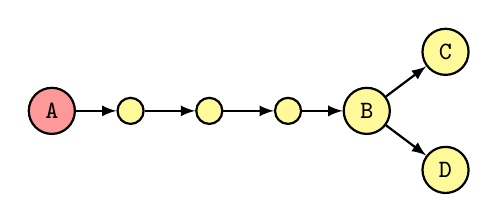
\begin{tikzpicture}
				\node[mynoder] at (0,0) (A) {A};
				\node[mynode] at (1,0) (u1) {};
				\node[mynode] at (2,0) (u2) {};
				\node[mynode] at (3,0) (u3) {};
				\node[mynode] at (4,0) (B) {B};
				\node[mynode] at (5,0.75) (C) {C};
				\node[mynode] at (5,-0.75) (D) {D};
				\path (A) edge [myedge] (u1);
				\path (u1) edge [myedge] (u2);
				\path (u2) edge [myedge] (u3);
				\path (u3) edge [myedge] (B);
				\path (B) edge [myedge] (C);
				\path (B) edge [myedge] (D);
			\end{tikzpicture}
\ifstandalone
		\end{subfigure}
	\end{figure}
\end{document}
\fi
